%%%%%%%%%%%%%%%%%%%%%%%%%%%%%%%%%%%%%%%%%%%%%%%%%%%%%%%%%%%%%%%%%%%%%%%%%%%%%%%%%%%%%%%%%%%%%%%%%%%%%%%%%%%%%%%%%

\UC{Modifica informazioni acquirente}
\label{modifica-informazioni-acquirente}

\begin{figure}[H]
    \centering
    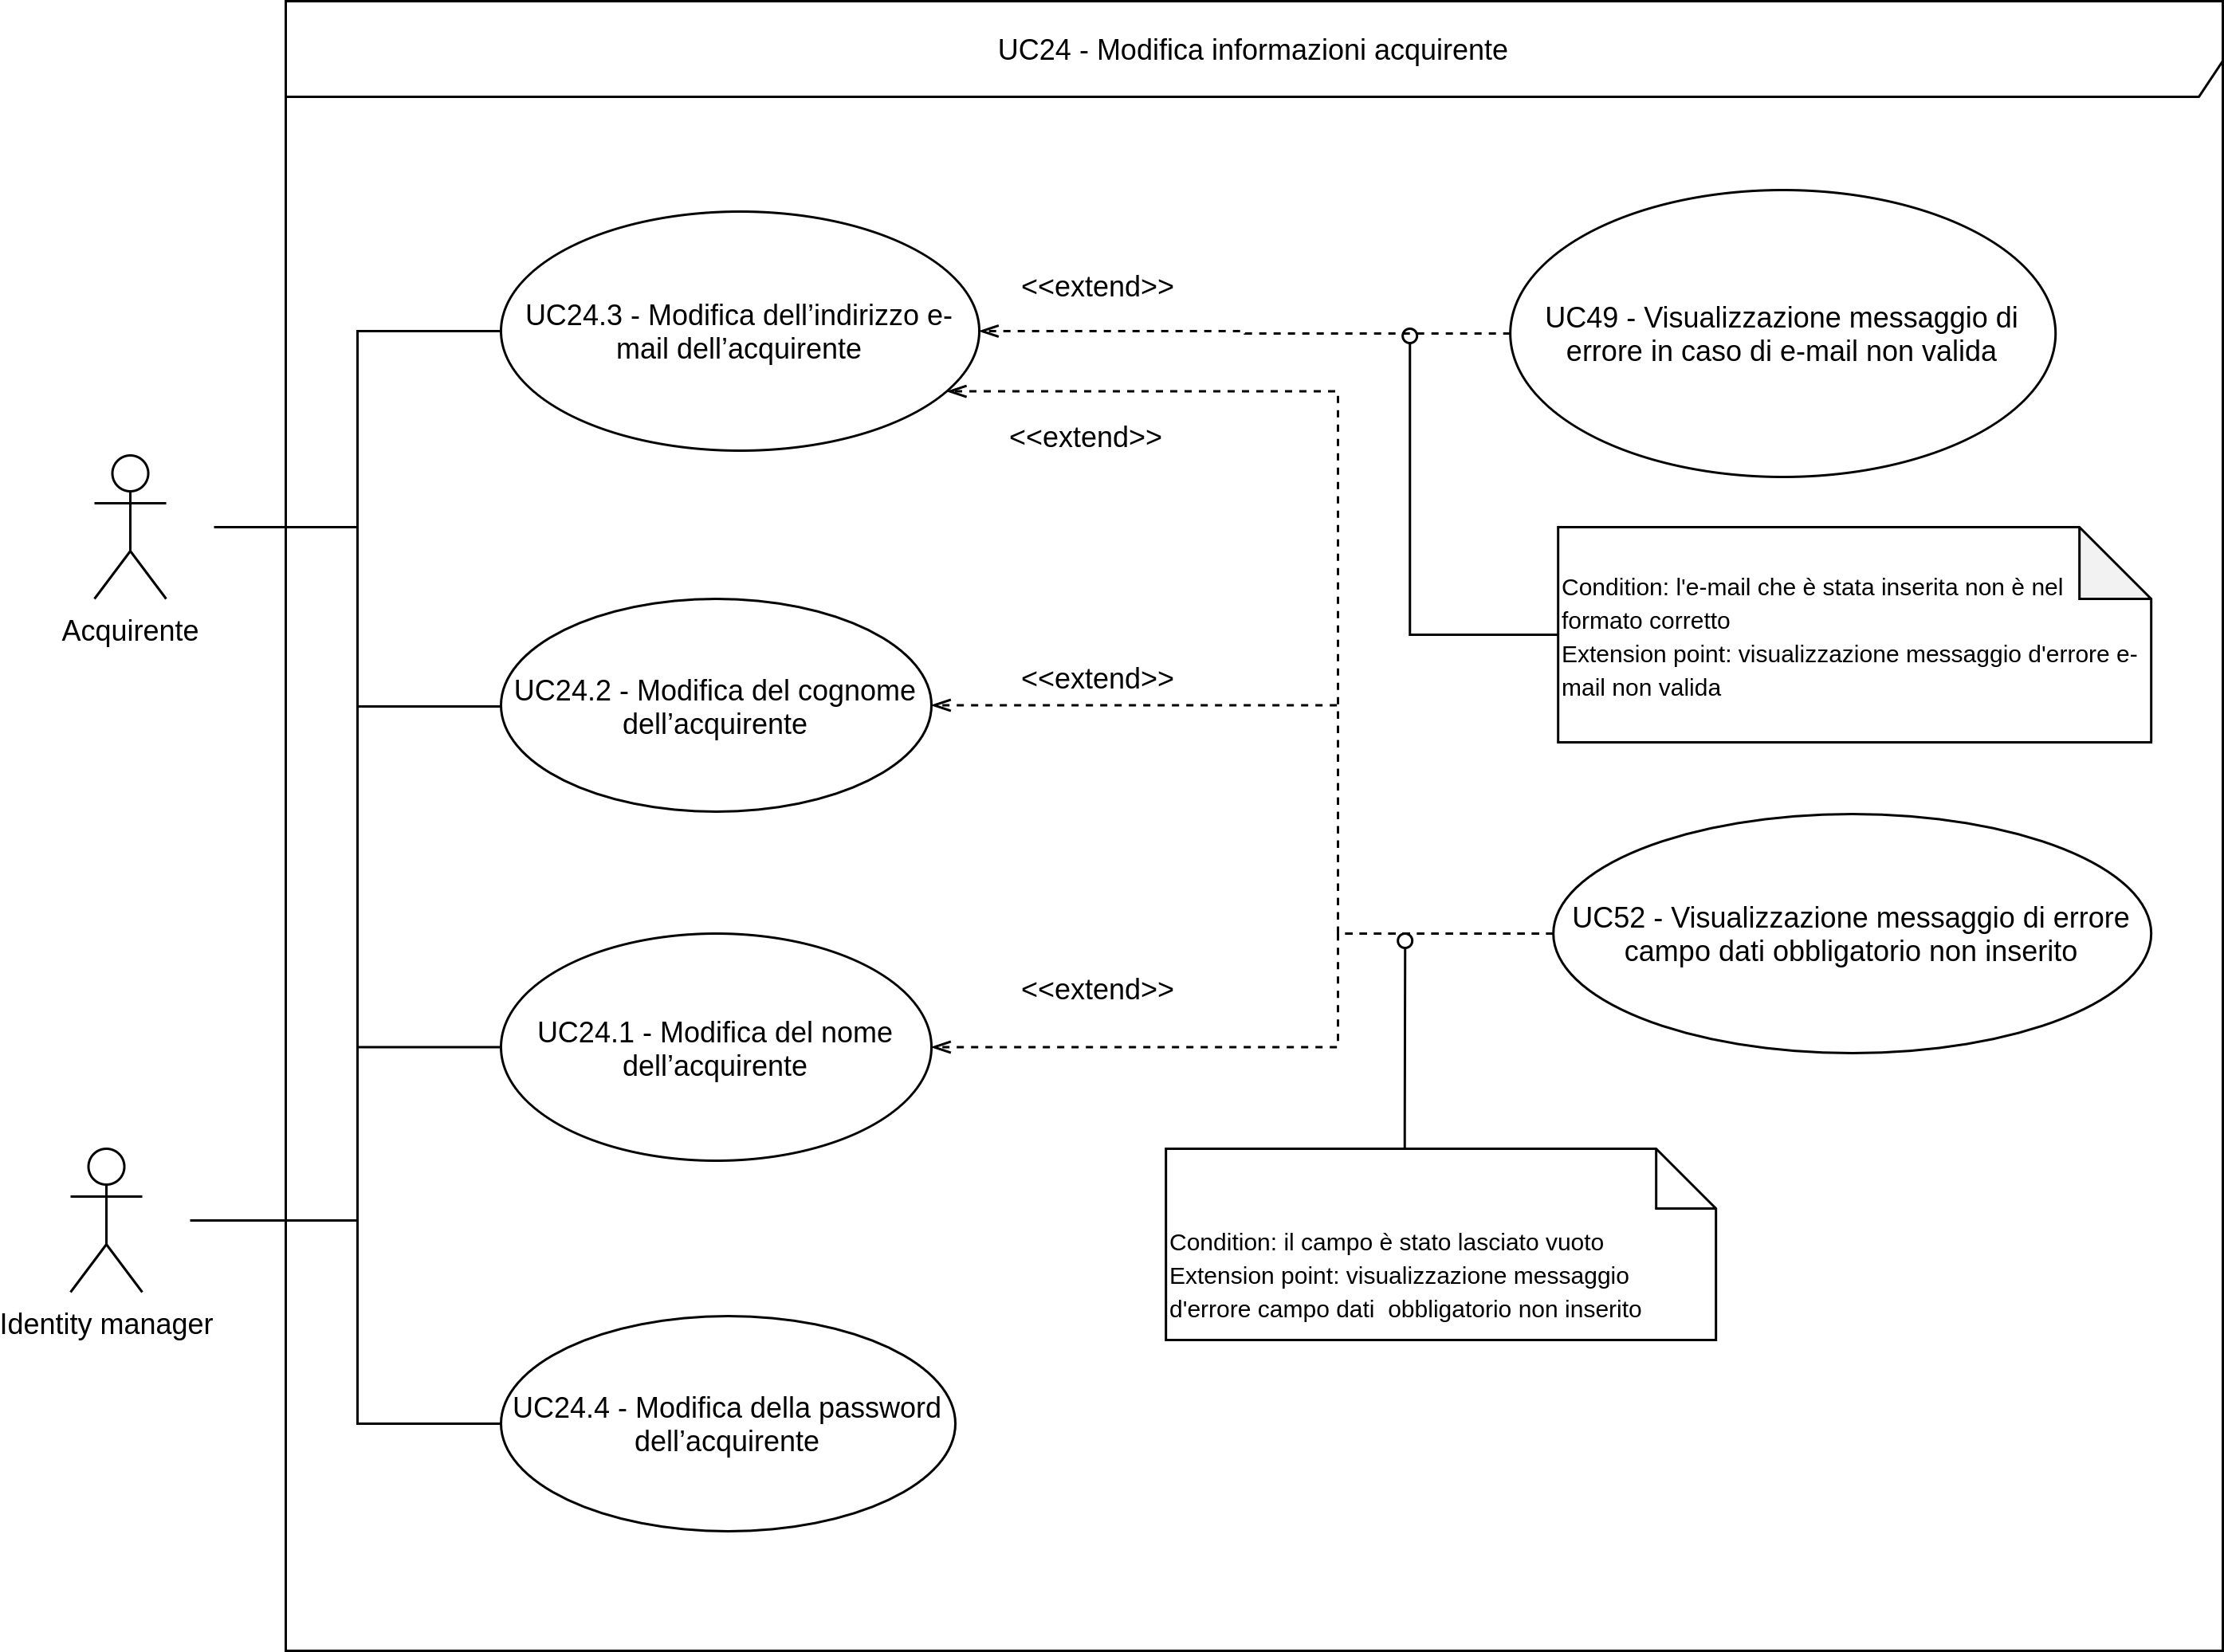
\includegraphics[scale=0.4]{Immagini/DiagrammiUC/Acquirente/ModificaInformazioniAcquirente.png}
    \caption{Diagramma di \actualUC: Modifica informazioni acquirente}
    \label{fig:modifica-informazioni-acquirente}
\end{figure}

L'acquirente può modificare le sue informazioni personali.
\begin{itemize}
    \item \textbf{Attori primari:} acquirente;
    \item \textbf{Attori secondari:} identity manager;
    \item \textbf{Precondizione:} l'acquirente si trova nella vista di modifica informazioni personali;
    \item \textbf{Postcondizione:} l'acquirente ha aggiornato le sue informazioni personali;
    \item \textbf{Scenario principale:} l'acquirente ha selezionato la funzionalità prevista per la modifica delle informazioni personali e, dopo aver compiuto la modifica, potrà confermarla attraverso la funzione di salvataggio. Le informazioni che si possono modificare sono:
    \begin{itemize}
        \item (UC\ref{modifica-informazioni-acquirente.nome}) - Modifica del nome dell'acquirente;
        \item (UC\ref{modifica-informazioni-acquirente.cognome}) - Modifica del cognome dell'acquirente;
        \item (UC\ref{modifica-informazioni-acquirente.email}) - Modifica dell'indirizzo e-mail dell'acquirente;
        \item (UC\ref{modifica-password}) - Modifica della password.
    \end{itemize}
    In seguito ci sarà la conferma delle modifiche compiute e le informazioni personali verranno modificate;
    \item \textbf{Scenari alternativi:}
    \begin{enumerate}[label=\lett]
        \item L'acquirente non conferma le modifiche effettuate, perciò non verranno modificate le informazioni personali.
    \end{enumerate}
    \item \textbf{Estensioni:} 
    \begin{enumerate}[label=\lett]
        \item L'acquirente modifica la propria e-mail con una già utilizzata nella piattaforma e l'identity manager lo segnala. In questo caso:
        \begin{itemize}
            \item L'identity manager segnala che le due password inserite non coincidono;
            \item (UC\ref{estensione:cambio-con-email-esistente}) - Verrà visualizzato il messaggio di errore in caso di cambio e-mail con una già utilizzata nella piattaforma;
            \item Verrà impedita la modifica delle informazioni.
        \end{itemize}
        \item L'acquirente inserisce una password di conferma diversa da quella inserita nel campo di inserimento nuova password e l'identity manager lo segnala. In questo caso:
        \begin{itemize}
            \item (UC\ref{estensione:password-conferma-diverse}) - Verrà visualizzato il messaggio di errore di password e password di conferma diverse;
            \item Verrà impedita la modifica delle informazioni.
        \end{itemize}
    \end{enumerate}
\end{itemize}

\subUC{Modifica del nome dell'acquirente}
\label{modifica-informazioni-acquirente.nome}

L'acquirente modifica il proprio nome.
\begin{itemize}
    \item \textbf{Attori primari:} acquirente;
    \item \textbf{Attori secondari:} identity manager;
    \item \textbf{Precondizione:} l'acquirente si trova nella schermata di modifica informazioni personali e vuole modificare il proprio nome;
    \item \textbf{Postcondizione:} l'acquirente ha aggiornato il proprio nome sulla piattaforma;
    \item \textbf{Scenario principale:} l'acquirente si trova nella schermata di modifica informazioni personali e vuole modificare il proprio nome attraverso le seguenti azioni:
        \begin{itemize}
            \item Si posiziona nel campo di inserimento del nome dove è presente quello attualmente utilizzata;
            \item Cambia il nome attuale modificandolo o inserendone uno completamente nuovo.
        \end{itemize}
    \item \textbf{Scenari alternativi:} 
    \begin{enumerate}[label=\lett]
        \item L'acquirente non modifica il proprio nome attuale e per questo non cambierà.
    \end{enumerate}
    \item \textbf{Estensioni:} 
    \begin{enumerate}[label=\lett]
        \item L'acquirente elimina il proprio nome attuale, non ne inserisce uno nuovo e l'identity manager lo segnala. In questo caso:
        \begin{itemize}
            \item (UC\ref{estensione:campo-obbligatorio-non-inserito}) - Verrà visualizzato il messaggio di errore campo dati obbligatorio non inserito;
            \item Verrà impedita la modifica delle informazioni.
        \end{itemize}
    \end{enumerate}
\end{itemize}

\subUC{Modifica del cognome dell'acquirente}
\label{modifica-informazioni-acquirente.cognome}

L'acquirente modifica il proprio cognome.
\begin{itemize}
    \item \textbf{Attori primari:} acquirente;
    \item \textbf{Attori secondari:} identity manager;
    \item \textbf{Precondizione:} l'acquirente si trova nella schermata di modifica informazioni personali e vuole modificare il proprio cognome;
    \item \textbf{Postcondizione:} l'acquirente ha aggiornato il proprio cognome sulla piattaforma;
    \item \textbf{Scenario principale:} l'acquirente si trova nella schermata di modifica informazioni personali e vuole modificare il proprio cognome attraverso le seguenti azioni:
        \begin{itemize}
            \item Si posiziona nel campo di inserimento del cognome dove è presente quello attualmente utilizzata;
            \item Cambia il cognome attuale modificandolo o inserendone uno completamente nuovo.
        \end{itemize}
    \item \textbf{Scenari alternativi:} 
    \begin{enumerate}[label=\lett]
        \item L'acquirente non modifica il proprio cognome attuale e per questo non cambierà.
    \end{enumerate}
    \item \textbf{Estensioni:} 
    \begin{enumerate}[label=\lett]
        \item L'acquirente elimina il proprio cognome attuale, non ne inserisce uno nuovo e l'identity manager lo segnala. In questo caso:
        \begin{itemize}
            \item (UC\ref{estensione:campo-obbligatorio-non-inserito}) - Verrà visualizzato il messaggio di errore campo dati obbligatorio non inserito;
            \item Verrà impedita la modifica delle informazioni.
        \end{itemize}
    \end{enumerate}
\end{itemize}

\subUC{Modifica dell'indirizzo e-mail dell'acquirente}
\label{modifica-informazioni-acquirente.email}

L'acquirente modifica la propria e-mail.
\begin{itemize}
    \item \textbf{Attori primari:} acquirente;
    \item \textbf{Attori secondari:} identity manager;
    \item \textbf{Precondizione:} l'acquirente si trova nella schermata di modifica informazioni personali e vuole modificare il proprio indirizzo e-mail;
    \item \textbf{Postcondizione:} l'acquirente ha aggiornato la sua e-mail;
    \item \textbf{Scenario principale:} l'acquirente si trova nella schermata di modifica informazioni personali e vuole modificare la propria e-mail attraverso le seguenti azioni:
        \begin{itemize}
            \item Si posiziona nel campo di inserimento dell'e-mail dove è presente quella attualmente utilizzata;
            \item Cambia l'e-mail attuale modificandola o inserendone una completamente nuova.
        \end{itemize}
    \item \textbf{Scenari alternativi:} 
    \begin{enumerate}[label=\lett]
        \item L'acquirente non modifica l'attuale indirizzo e-mail utilizzato e per questo non cambierà.
    \end{enumerate}
    \item \textbf{Estensioni:} 
    \begin{enumerate}[label=\lett]
        \item L'acquirente modifica la propria e-mail con una non valida e l'identity manager lo segnala. In questo caso:
        \begin{itemize}
            \item (UC\ref{estensione:email-non-valida}) - Verrà visualizzato un messaggio di errore in caso di e-mail non valida;
            \item Verrà impedita la modifica delle informazioni.
        \end{itemize}
        \item L'acquirente elimina la propria e-mail attuale, non ne inserisce una nuova e l'identity manager lo segnala. In questo caso:
        \begin{itemize}
            \item (UC\ref{estensione:campo-obbligatorio-non-inserito}) - Verrà visualizzato il messaggio di errore campo dati obbligatorio non inserito;
            \item Verrà impedita la modifica delle informazioni.
        \end{itemize}
    \end{enumerate}
\end{itemize}

%%%%%%%%%%%%%%%%%%%%%%%%%%%%%%%%%%%%%%%%%%%%%%%%%%%%%%%%%%%%%%%%%%%%%%%%%%%%%%%%%%%%%%%%%%%%%%%%%%%%%%%%%%%%

\UC{Eliminazione account dell'acquirente}
\label{eliminazione-account-acquirente}

L'acquirente può eliminare il proprio account.
\begin{itemize}
    \item \textbf{Attori primari:} acquirente;
    \item \textbf{Precondizione:} l'acquirente si trova nella schermata personale e ha selezionato l'azione di eliminazione del proprio account;
    \item \textbf{Postcondizione:} l'account dell'acquirente non è più presente nella piattaforma;
    \item \textbf{Scenario principale:} l'acquirente si trova nella schermata personale e ha selezionato la funzionalità di eliminazione del proprio account. In seguito verrà visualizzato un messaggio di conferma dell'operazione e, se l'acquirente conferma, viene eliminato l'account;
    \item \textbf{Scenari alternativi:}
    \begin{enumerate}[label=\lett]
        \item Se non conferma viene riportato alla propria schermata personale e l'account non viene eliminato.
    \end{enumerate}.
\end{itemize}
